\documentclass[11pt]{article}
\usepackage[utf8]{inputenc}
\usepackage[english]{babel}
\usepackage{bilal2vec}

\title{CS 341 - Solutions}
\author{Bilal Khan\\
\href{mailto:bilal2vec@gmail.com}{bilal2vec@gmail.com}}
\date{\today}

\begin{document}

\maketitle

\tableofcontents

\section{1}

Your folder contains 4 ciphertexts, each of which is an encryption of some English plaintext written in a similar style of text. The plaintext may start in the middle of a sentence and may end in the middle of a word. Each plaintext is different and each is encrypted with a different cipher. The four ciphers used, in random order in your set, are:

• shift cipher
• substitution cipher
• Vigen`ere cipher, for an unknown block length between 6 and 13
• transposition cipher, for an unknown block length between 6 and 13

Your task is to determine which cipher was used for each ciphertext, and what the corresponding plaintext is, using the following steps. You may write software to do so in any language of your choice, or use online tools to assist, but please indicate which tool(s) you used. If you write your own software to help you solve, please include that in your submission.

\subsection{a}

For each ciphertext, using either a table or a histogram, present the single character
frequencies and a description of the relevant properties of the single character frequencies.

\begin{table}[h]
    \centering
    \begin{tabular}{|c|c|c|c|c|c|c|c|c|c|c|c|c|c|c|c|}
    \hline
    Ciphertext & A & B & C & D & E & F & G & H & I & J & K & L & M \\
    \hline
    0 & 20 & 72 & 58 & 14 & 22 & 52 & 34 & 15 & 36 & 41 & 45 & 37 & 65 \\
    \hline
    1 & 12 & 39 & 0 & 20 & 0 & 98 & 14 & 18 & 46 & 122 & 23 & 26 & 74 \\
    \hline
    2 & 81 & 14 & 13 & 56 & 143 & 16 & 23 & 71 & 69 & 1 & 10 & 51 & 13 \\
    \hline
    3 & 16 & 0 & 0 & 30 & 17 & 85 & 133 & 23 & 31 & 71 & 54 & 27 & 72 \\
    \hline
    \end{tabular}
    \caption{Character frequencies in ciphertexts (A-M)}
    \label{tab:char_frequencies_A_M}
    \end{table}
    
    \begin{table}[h]
    \centering
    \begin{tabular}{|c|c|c|c|c|c|c|c|c|c|c|c|c|c|c|c|}
    \hline
    Ciphertext & N & O & P & Q & R & S & T & U & V & W & X & Y & Z \\
    \hline
    0 & 35 & 21 & 41 & 43 & 41 & 32 & 32 & 30 & 40 & 39 & 31 & 71 & 33 \\
    \hline
    1 & 71 & 0 & 9 & 58 & 21 & 64 & 68 & 8 & 0 & 42 & 59 & 91 & 17 \\
    \hline
    2 & 69 & 64 & 14 & 0 & 45 & 72 & 80 & 25 & 14 & 31 & 1 & 24 & 0 \\
    \hline
    3 & 63 & 7 & 37 & 1 & 0 & 10 & 73 & 45 & 113 & 11 & 57 & 7 & 17 \\
    \hline
    \end{tabular}
    \caption{Character frequencies in ciphertexts (N-Z)}
    \label{tab:char_frequencies_N_Z}
    \end{table}

    \begin{figure}[h]
        \centering
        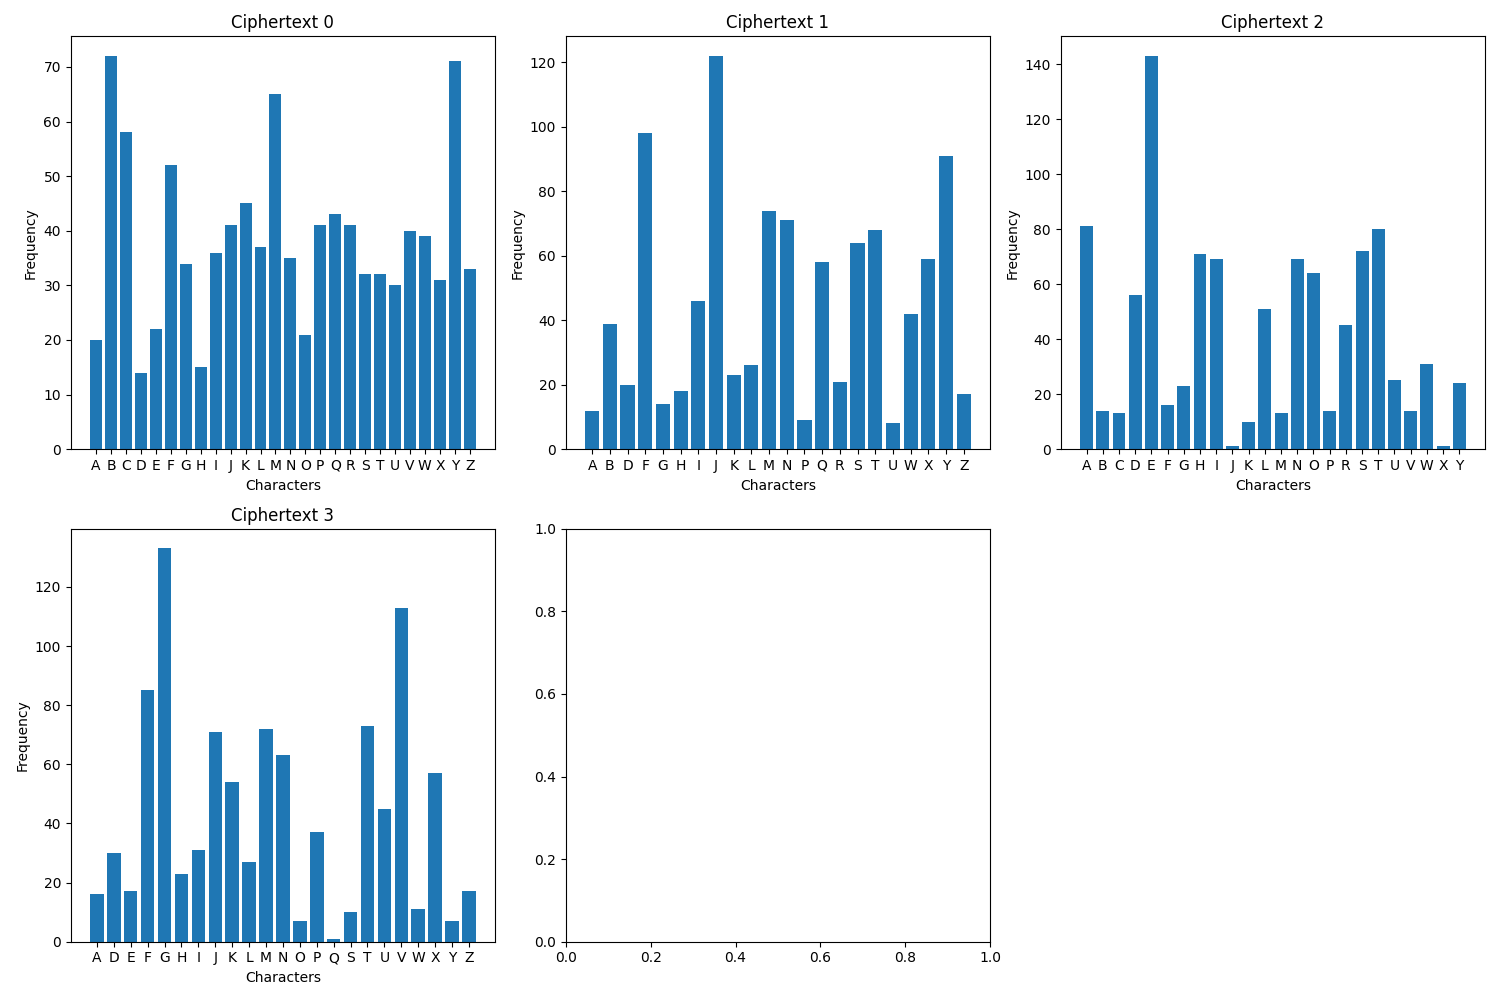
\includegraphics[width=400px]{Figure_1.png}
        \caption{Your caption here} % Optional: Add a caption for the figure
        \label{fig:your_label} % Optional: Add a label for referencing
    \end{figure}


    Ciphertext 0 has relatively uniform character frequencies

    Ciphertext 1 has character frequences similar to that of english but permuted from what we'd expect.

    Ciphertext 2 has character frequencies with higher peaks and lower valleys than english.

    Ciphertext 3 has character frequencies that are very similar to english but shifted to the right.
    
   
\subsection{b}

Explain clearly how the single character frequencies are expected to look for the ciphertext from each of the four cipher algorithms used. Use the experimental observations from part (a) to argue which ciphertext comes from which of the four ciphers.

Ciphertext 1 is likely a shift cipher. The two most frequent characters are J and F, which are 5 shifts away from E and A, two of the most frequent characters in English.

Ciphertext 3 is likely a substitution cipher. Its two most frequent characters, G and V appear in the same frequency as E and T in english, but at different offsets from each other, indicating that the alphabet has been permuted.

Ciphertext 2 is likely a transposition cipher since the character frequencies match that of english, so only the order of characters has been changed.

Ciphertext 0 is likely a vigenere cipher since its character frequences have been smoothed out to be relatively uniform compared to english.
    
\subsection{c}

Explain, with direct reference to the statistics that you found, the procedure you can use to cryptanalyze each cipher. You are not expected to perform the cryptanalysis in this part you need to explain how it can be done in principle for each type of cipher and how the measured statistics can help.

For the shift cipher, compare the frequency of each character in the ciphertext to the expected frequency of enlglish text. The shift of the most frequent char in the ciphertext should be the shift from E in english to E in the ciphertext.

For the substitution cipher, compare the frequncy of each character in the ciphetext ot the expected frequency of english text. The most frequent chars in the ciphertext should correspond exactly to the frequent chars in english, and you can simply permute the ciphertext frequency to get the key.

For the transposition cipher, you will notice that the frequency histogram should exactly match the english histogram. You would need to try all possible keys for all possible block lengths to decode the plaintext.

For the vigenere cipher, try all possible block lengths and for each block length, use a frequency histogram of the all the ith chars of all blocks of the ciphertext and compare if the relative frequncies match english. If so, the block length has been found and you can use the shifts between the most freq char in the histogram vs english to find the key.

\subsection{d}

Using whatever technique or tools you like, obtain the key and plaintext for the ciphertexts encrypted using the shift, substitution, and Vigen`ere cipher. It is okay if you only give the first 50 or so characters of the plaintext. It is okay if the first or last few characters of your plaintext are nonsensical, as the plaintext may have been interrupted in the middle of a word and may not be a multiple of the block length

Ciphertext 0: Tool: https://www.boxentriq.com/code-breaking/vigenere-cipher key: oifygyrxu Plaintext:

de said he to the father have you no other daughters no 

Ciphertext 1: Key = 5, Plaintext:

GECOMEINCOMEINSAIDSHEISNOTTHISMUCHBETTERTHANTHEFILTHY

Ciphertext 3: tool: https://www.guballa.de/substitution-solver Key = "cxjgyheuwndmasklqzportbivf", Plaintext:

LEARNTSOMELITTLEMATTERSTHATAREYETUNKNOWNTOMESOTHESTUDENTS


\subsection{e}

Suppose that, instead of using only one cipher, we decided to combine two ciphers with independent keys, by encrypting the message using the first cipher, and then encrypting that ciphertext using the second cipher. For each of the following explain why you could still break the combination.

i. Shift cipher followed by substitution cipher.

Permuting the shifted characters of the shift cipher by a fixed alphabet permutation mapping will still maintain the original english character frequencies of characters in the ciphertext. We can still guess that the ith most frequent char in the ciphertext is the ith most frequent char in english and break the combination just as easily as the substitution cipher.

ii. Substitution cipher followed by Vigenere cipher

We can still determine the block length by sweeping over block lengths and seeing which block length has the closest match in sorted character frequencies since the substituion cipher will only reorder char freqs. After that, the block-size-length number of frequency analyses that we do to crack vigenere will still work since vigenere will add a constant shift to each char in every group and the substituion cipher will permute the chars in each group. Both of these operations preserve the relative differences of english text in character frequencies in each group.


\section{2}

The affine cipher is a symmetric key encryption scheme with the following properties: The plaintext space and ciphertext space is $Z_{26}$, the set of integers modulo 26. The key space is the set of all pairs (a, b) where a and b are elements of $Z_{26}$ such that $\gcd(a, 26) = 1$. The encryption function is $E_k(m) = am + b \mod 26$, where the key is k = (a, b). The decryption function is $D_k(c) = a^{-1}(c - b) \mod 26$ where the key is k = (a, b). 

Recall: For an element a modulo n, the inverse $a^{-1}$ of a is an element of $\mathbb{Z}_n$ such that $a \times a^{-1} \equiv 1 \mod n$. An inverse exists if and only if gcd(a, n) = 1, in which case the inverse is unique modulo n. In practice, computing the inverse modulo n of a can be done efficiently, even if a and n are very large

\subsection{a}  What is the size of the keyspace of the affine cipher?

All valid $a$ are coprime to $26$. The prime factors of $26$ is $2$ and $13$. Therefore, of all numbers between $1$ and $26$, $1,3,5,7,9,11,15,17,19,21,23,25$ are valid $a$. There are $12$ such numbers. $b$ can be any number between $0$ and $25$ so there are $26$ choices for $b$. Therefore, the size of the keyspace is $12 \times 26 = 312$.

\subsection{b} Given a single plaintext-ciphertext pair (m, c), how many keys k are there such that c = Ek(m)?

\begin{align*}
    c &\equiv am + b \mod 26 \\
    c - am &\equiv b \mod 26
\end{align*}

For a fixed $c$ and $m$, and for every valid $a$ there is a $b$ that satisfies the equation, and that $b$ is unique because it must be equal to $c - am$ mod $26$ with $b$ in the range $0$ to $25$. There are $12$ choices of $a$ so there are $12$ keys. 

\subsection{c} Suppose that you are allowed to carry out a chosen plaintext attack where you are allowed to have at most two plaintexts encrypted. Explain how you could recover the secret key

\begin{align*}
    c_1 &= am_1 + b \mod 26 \\
    c_2 &= am_2 + b \mod 26 \\
    c_1 - c_2 &= a(m_1 - m_2) \mod 26 \\
    (c_1 - c_2) (m_1 - m_2)^{-1} &\equiv a \mod 26
\end{align*}

We cand do the above to find $a$. To find $b$, we can substitute $a$:

\begin{align*}
    c_1 &= am_1 + b \mod 26 \\
    b &= c_1 - am_1 \mod 26
\end{align*}

\subsection{d} Since the affine cipher is not secure against message recovery under chosen plaintext
attacks, let's try to salvage it by working in a large modulo, say a large prime $p > 2^{256}$. The
new scheme becomes:

The plaintext space and ciphertext space is $\mathbb{Z}_p$, the set of integers modulo $p$.
The key space is the set of all pairs (a, b) where a and b are elements of $\mathbb{Z}_p$ such that $\gcd(a, p) = 1$.
The encryption function is $E_k(m) = am + b \mod p$, where the key is k = (a, b).
The decryption function is $D_k(c) = a^{-1}(c - b) \mod p$, where the key is k = (a, b).

Is the new scheme secure against an exhaustive key search attack?
Is the new scheme secure against a chosen plaintext attack? Explain why or why not.

The new key space is much larger. $p$ is a large prime $> 2^{256}$ so all choices of $a$ in that range are coprime to $p$ and valid. Combined with $b$, this means the key space is of size $(2^{256})^2 = 2^{512}$ and is sufficiently large to not be brute forcable.

The new scheme is not secure agaisnt a CPA, and the inverse operation is still efficient, so the same attack from above will work.

\subsection{e} In addition to using large numbers, what if we decided to double encrypt? The new
scheme becomes:

• The plaintext space and ciphertext space is $Z_p$, the set of integers modulo p.

• The keys $k_1, k_2$ are two random pairs (a1, b1), (a2, b2) where a1, a2 and b1, b2 are random elements of Zp such that $\gcd(a_1, p) = \gcd(a_2, p) = 1$.

• The encryption function is $E_{k2} (E_{k1} (m)) = a_2(a_1 m + b_1) + b_2 \mod p$.

• The decryption function is $D_{k1} (D_{k2} (c)) = a^{-1}_1 (a^{-1}_2 (c - b_2) - b_1) \mod p$.

Is this double-encrypted affine cipher secure against a chosen plaintext attack?

No. We can simplify the encryption function to be:

\begin{align*}
    E_{k2}(E_{k1}(m)) &= a_2(a_1 m + b_1) + b_2 \mod p \\
    &= a_2 a_1 m + (a_2 b_1 + b_2) \mod p
\end{align*}

$a_2 a_1$ and $a_2 b_1 + b_2$ are constants for a given set of two key pairs and can be viewed as a single affine cipher, with the same vulnerability.

\section{3}

Most programming languages include pseudorandom bit generators so that users can generate random numbers. For example, the C programming language has the rand() function, and Java has the java.util.Random class. Both of these functions, as well as analogous functions in many other programming languages use a function called a linear congruential generator (LCG), which is constructed as follows.

A modulus M is fixed as part of the specification of the system.

• The seed key k is a triple (a, b, $X_0$) where a and b are random elements of $Z_M$ such that $\gcd(a, M ) = 1$ and $X_0$ is a random element of $Z_M$.

• The initialization function for the pseudorandom bit generator saves (a, b, $X_0$) as the initial state.

• The update and output function for the pseudorandom bit generator takes as input a state (a, b, $X_i$) (starting with $i = 0$), and produces an output state (a, b, $X_{i+1}$) where $X_{i+1}$ = $a X_i + b \mod M$, and outputs $X_{i+1}$ as the next partial output of the pseudorandom generator.

Suppose we used the LCG to construct a symmetric key encryption scheme as follows. Fix modulus
$M = 26$. Let the plaintext space and ciphertext space be $\{A, \cdots , Z\}^\star$, in other words arbitrary-length strings of English letters. The encryption key is a randomly chosen seed key satisfying the conditions above. The encryption algorithm is as follows:

$E_k(m)$

$for i = \cdots |m|:$

$X_i \leftarrow a X_{i-1} + b \mod 26$

$c_i \leftarrow m_i + X_i \mod 26$

$return c = (c_1, \cdots, c_{|m|})$

\subsection{a} Write psuedocode for the decryption algorithm

\begin{algorithm}[]
    $m \leftarrow$ ""\;
    $X \leftarrow X_0$\;
    \For{$i \leftarrow 1$ \KwTo $|m|$}{
        $X \leftarrow aX + b \mod 26$\;
        $m_i \leftarrow c_i - X \mod 26$\;
    }
    \Return{$m$}
\end{algorithm}

\subsection{b} Is this scheme secure against a chosen plaintext attack? If so, explain why. Otherwise, propose an attack.

No it is not secure. Given a plaintext of our choice, we can deduce the values of $X_i$, $a,b$. Choose the input to be a string of $A$s ($m_i = A = 0 \mod 26$). $C_i$ will then be equal to $X_i$. We can pass in a sequence of $m_i = 0$s to get a system of equations for $X_i = aX_{i-1} + b \mod 26$. Solve the system of equations to get $a,b$.

\subsection{c} Would the scheme be secure if we worked with a larger modulus say $M$ being a prime larger than $2^{256}$

No, this attack would still work. Using a larger modulus would not change the validity of using a string of $A$s that get mapped to $0$s in the ciphertext and using that to solve for $a,b$.

When programming any kind of security-related code, you should make sure that you are using a cryptographically secure pseudorandom number generator, rather than a weak pseudorandom number generator like the one described above. Carefully check your programming language's documentation to find out what functions are cryptographically secure pseudorandom number generators and how to use them safely. For example,

In Java: Use java.util.SecureRandom instead of java.util.Random.

• In Python: Use the secrets module instead of the random module.

• In C: Use an external library like OpenSSL or on Unix carefully read from /dev/urandom, instead of using rand()

\section{4} Substitution Permutation Networks.

As you know, there is an intense rivalry between math and engineering students at the University of Waterloo. A plot is underway to steal Math Orientation's 40-foot tall pink tie by a secretive sub-committee of the Engineering Society called the Awesome Engineering Squad (AES). In order to plan their dastardly plots, the Awesome Engineering Squad has decided to encrypt all of their communications.

However, the leader of the AES (who, it should be noted, has not taken CO 487) was recently told by a psychic that a disastrous attack on substitution permutation networks was on the horizon, since permutations are so easy to reverse. Consequently, the leaders of the AES have decided to take matters into their own hands, and create a new cipher: NVP (Not Very Permute-y). The NVP cipher works just like an substitution-permutation network, except each permutation is replaced with more S-boxes, so that the resulting cipher looks something like this:

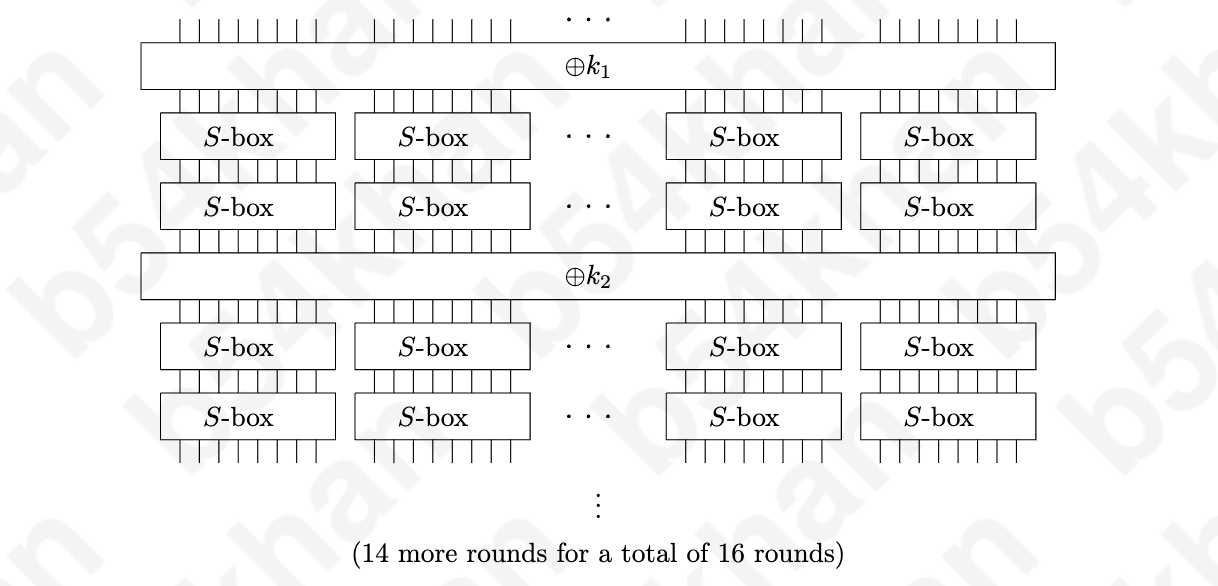
\includegraphics[width=400px]{a1q4.png}

It takes as input a 128-bit message block and a 128-bit key, and outputs a 128-bit ciphertext. It expands the 128-bit key into sixteen 128-bit round keys $k_1, \cdots, k_{16}$. It has 16 rounds. In each  round $i = 1, \cdots, 16$:

• the round key $k_i$ is XORed into the state,

• then the bits are sent through the S-boxes in groups of 8,

• then the bits are sent through the S-boxes AGAIN, still in groups of 8.

Note that all the S-boxes are the same substitution.

\subsection{a} [4 marks] Describe how an adversary can totally break the NVP cipher under a chosen plaintext attack using significantly fewer operations than exhaustive key search would.

The weakness is in the absence of permutation layers between sbox layers. This means that every application of the cipher to a 128 bit block with its 128 bit key can be broken up into 16 independent applications of the cipher to 8 bit blocks with their 8 bit keys.

Since the sbox permutations are known, we can generate all possible 8 bit ciphertexts for all possible plaintext values ($2^k = 256$ values) for each group independently and in parallel.

The range of keys we need to search over is reduced from $2^{128}$ to $16$ independent searches over $2^8$ keys. Each of these searches can be done in parallel. Brute force all $256$ keys for each of the 16 blocks in parallel and match against the known plaintext-ciphetext pairs. 

\subsection{b} [2 marks] Would adding more rounds help? Why or why not?

No, the keyspace per block remains the same, increasing the numeber of rounds would only increase runime linearly.

\subsection{c} [2 marks] What would be the effect of using S-boxes which are 128 bits wide, compared to 8 bits wide? Why is this not done in practice?

Wider sboxes would make this attack infeasible since the block size will increase to $2^{128}$ and increase the key space to $2^{128}$ as well.

A wider sbox is infeasible because you would need to store a substition table of size $2^{128} \times 2^{128}$ which is impossible from a storage perspective.


\section{5}

The Engima machine and IND-CPA security. Perhaps the most famous cipher is the Enigma code, used by the Germans in WWII. Encryption and decryption were performed using a device called the Enigma machine. Very generally speaking, the Enigma machine is arranged as follows, where each line represents an electrical wire:

When the Enigma machine is configured, it forms a circuit leading from the keys on the keyboard to the lamps on the lampboard. When an Axis member wishes to encrypt a letter, they type that key, which sends current flowing through the plugboard, the rotors, the reflector, back through the rotors, back through the plugboard, and finally to the lampboard, where the lamp corresponding to the encryption of that letter will light up. For this symmetric key cryptosystem, the secret key is the choice of rotors (there are many different rotor options, but Enigma machines only use three at a time), and the wiring of the rotors, plugboard, and reflector. Randomness is introduced by the operator (who is encrypting a message) by choosing the initial position of the rotors. This should be different for every message, and the settings are sent in the clear before the encrypted ciphertext is sent. For a more detailed description of each component:

Keyboard: This consists of the 26 letters of the alphabet, and is the part of the machine which takes input. Axis members encrypt messages letter-by-letter, by pressing the key corresponding to each letter they wish to encrypt.

• Plugboard: This swaps certain letters, in a way determined by the secret key. In most configurations, 10 pairs of letters were chosen (the letters in each pair were swapped with each other), and the remaining 6 letters were left untouched.

• Rotors: Each individual rotor works as a substitution cipher. However, they have the ability to rotate, and (some) rotors do so each time a new key is pressed. Together, they form a polyal- phabetic substitution cipher 2 which is very difficult (not impossible, but very time-consuming) to crack by brute force. It is important to note that, due to the multiple substitution alphabets, it might be the case that multiple instances of the same letter in a word are mapped to different letters by the encryption function, and that two different letters in the word are mapped to the same letter by the encryption function.

• Reflector: This pairs up the 26 letters of the alphabet, and connects each pair with a wire to send the current back through the rotors and plugboard along a different path than the one it came from. The main purpose of the reflector is to give Enigma the property that encryption is its own inverse — that is, decryption can be performed by running the encryption algorithm on a ciphertext (under the same settings that it was encrypted under). This was a very desirable property for convenience and practicality reasons.

• Lampboard: This consists of 26 lamps, each corresponding to a letter of the alphabet. The circuit formed by the plugboard, rotors, and reflector connects every key on the keyboard to exactly one lamp on the lampboard (namely, the one which corresponds to the encryption of the key pressed), and this lamp lights up when its corresponding key is pressed.

\subsection{a} Which of the following are possible encryptions of the message “STEBILA”? That is, for which of the following could there exist a secret key such that the encryption of “STEBILA” on an Enigma machine configured in the way specified by the key, would produce the ciphertext listed? Give a brief explanation in each case (you can group answers with the same explanation together).

(i) ESTUPINAN

(ii) MOKRANI

(iii) RIVERA

(iv) REYNES

(v) STECKEL

(vi) SWANSON

(vii) GOOOOSE

Hint: There should be three categories: POSSIBLE, IMPOSSIBLE because reason X, IMPOSSIBLE because reason Y, and reasons X and Y should have very different flavours.

POSSIBLE: (ii), (vii)

IMPOSSIBLE because length is wrong (not 7): (i), (iii), (iv)

Impossible because letter is mapped to itself: (v), (vi)

Enigma reflection property means that encryption is its own inverse, so any letters mapping to themselves would break encryption being secure.

\subsection{b}

[3 marks] Show that Enigma does not satisfy IND-CPA security. To do this, you must write an adversary which can win the IND-CPA security experiment on this cryptosystem with probability noticeably greater than $1/2$ (and justify why this is the case). You may assume that every possible encryption of a letter occurs with equal probability.

\end{document}